% !TEX root = /Users/Gela/Desktop/Thesis_latex/thesis.tex

\section{Semi-permeable membrane}
\label{membrane}
A membrane is defined as a barrier between two homogeneous phases. The process is a continuos steady-state operation consisting three streams: feed, permeate and reject. Main concern in the process boundary is the semipermeable barrier that selectively allows the passage of some components but not others. \cite{Singh}

\section{Osmosis} 
\label{osmosis}
The osmosis process occurs when two solutions of different chemical concentration are separated by a semi-permeable membrane. The two different solutions will try to reach equilibrium. The solution with less concentration will have a natural tendency to migrate through the membrane over to the side with higher concentration.  
Osmosis is a naturally occurring phenomenon and one of the most important processes in nature. The pressure that occurs is called the osmotic pressure. The phenomenon can be seen in Figure \ref{fig:osmosis}

\begin{figure}[h]
    \centering
    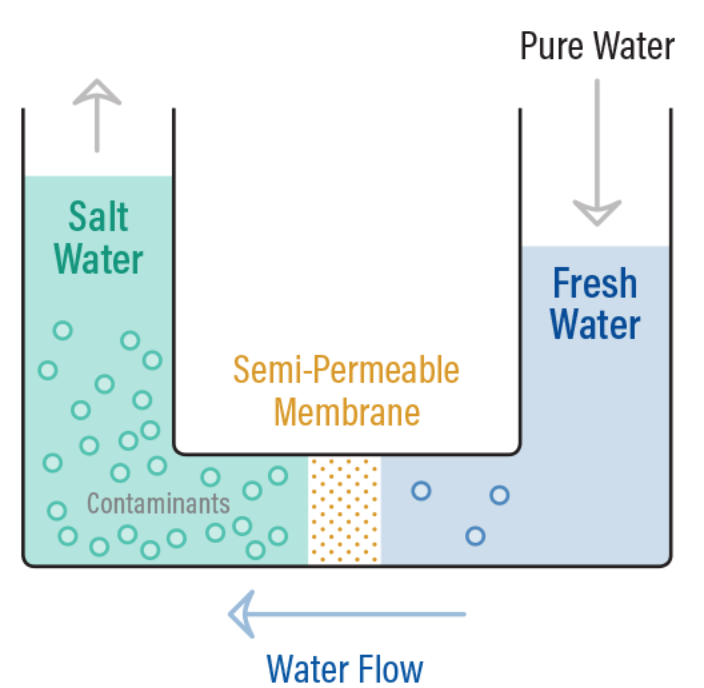
\includegraphics[width=0.4\textwidth]{Osmosis}
    \caption{Osmosis}
    \label{fig:osmosis}
\end{figure}

\section{Reverse osmosis}
\label{RO}
The reverse osmosis(RO) process is the reverse process of the osmosis. When pressure is applied to a semipermeable membrane, the water molecules are forced through the semipermeable membrane and the contaminants are not allowed true. The amount of pressure required depends on the salt concentration of the water. In order to gain reverse osmosis the pressure applied must be greater than the osmosis pressure. The membrane employs cross filtration rather than standard filtration. With cross filtration, the solution passes through the filter with two outlets. One solution passes true the membrane and is called permeate and is the filtered solution. The other solution can be drained or be fed back into the filtering system. The contaminants build up att the surface area and it is of great importance to try to sweep them away and hold the surface clean. If the contaminants builds up the performance of the membrane will decrease, and cleaning with chemicals or heat water might be necessary\cite{Puretech}. The phenomenon of reverse osmosis can be seen in \ref{fig:ReverseOsmosis}.
\begin{figure}[h]
    \centering
    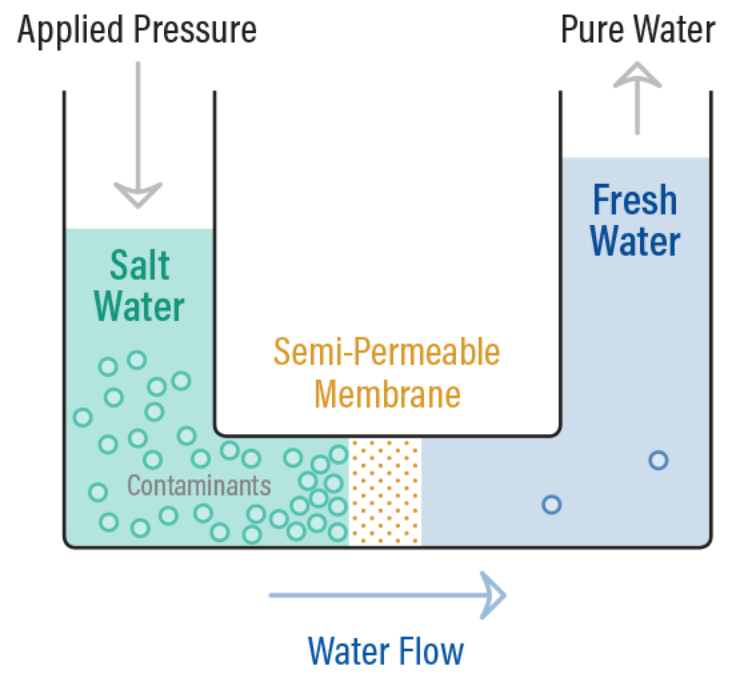
\includegraphics[width=0.4\textwidth]{ReverseOsmosis}
    \caption{Reverse Osmosis}
    \label{fig:ReverseOsmosis}
\end{figure}
In order to obtain good performace over the RO membrane there are some parameters that should be taken in consideration when designing a RO system. These are:

\begin{labeling}{alligator}
\renewcommand\labelitemi{ }
\item [Pressure:]  feed ($P_{f}$), permeate ($P_{p}$), reject, ($P_{r}$)
\item [Conductivity:] feed, $C_{f}$, permeate ($C_{p}$), reject ($C_{r}$)
\item [Flow:] feed ($Q_{f}$), permeate ($Q_{p}$), reject($Q_{r}$)
\item [Temperature:] feed ($T_{f}$), permeate ($T_{p}$), reject ($T_{r}$)
\end{labeling}


\subsection{Fouling}
Fouling occurs when contaminants accumulate on the surface of the membrane. The fouling contributes to a pressure drop that will decrease the performance of the membrane and cause less permeate flow. Fouling will happen eventually to some extent given the fine pore size of the membrane. A high reject flow and proper pretreatment will extend the operational time between cleaning procedures of the membrane\cite{Puretech}. 

\section{Mathematical modeling of reverse osmosis} 
\label{soldiff}
There are different models to describe the flow of solutes and solvents in the reverse osmosis process. The mass balance equations are central in modeling the process. Figure \ref{fig:ReverseOsmosis} shows the main process. \\

A hydraulic pressure is applied to to the feed stream of concentration, $C_{f}$ and results in a flow rate $Q_{f}$. Some of the solvent, pure water, passes through the RO-membrane  characterized by solvent permeability, solute permeability and surface area. The product water (purified water), is called permeate and has the concentration $C_p$ and flow $Q_p$. The concentration, called reject has the concentration $C_r$ with flow $Q_r$. The study objective of this basic RO-modeling is to calculate output concentrations and flow rates in terms of input and operation conditions. Parameters used to evaluate the performance of the RO-membrane is rejection ratio:
\begin{equation}
\label{eq:rejection}
R=1-\frac{C_{p}}{C_{f}}
\end{equation}
and recovery ratio:

\begin{equation}
\label{eq:recovery}
Y=\frac{Q_{p}}{Q_{f}}
\end{equation}
which express the quality and quantity of the solvent product respectively. 
\\Mass balance in the system gives:

\begin{equation}
\label{eq:feedflow}
Q_{f}=Q_{p}+Q_{r}
\end{equation}
and:

\begin{equation}
\label{eq:mass}
C_{f}Q_{f}=C_{p}Q_{p}+C_{r}Q_{r}
\end{equation}
Solvent flux per unit time per unit membrane surface area is described by:

\begin{equation}
\label{eq:flux}
J_{w}=\frac{Q_{p}}{A_{m}}= A(\Delta P - \Delta \pi)
\end{equation}
where $\Delta\pi = \pi_{f} - \pi_{p}$ is the osmotic pressure difference between feed and permeate side and $A_{m}$ is membrane surface area.
Solute flux is given by:

\begin{equation}
\label{eq:solflux}
J_{s}=B(C_{f}- C_{p})
\end{equation}
 where B is the solute permeability.
\\The permeate concentration can be described by:

\begin{equation}
\label{eq:permcond}
C_{p}=\frac{C_{f}}{1+\frac{A}{B}(\Delta P - \Delta\pi)}
\end{equation}
where A is solvent permeability.
Permeate flow is described by:

\begin{equation}
\label{eq:permflow}
Q_{p}=Q_{f}Y
\end{equation}

The four mass balance equations (\ref{eq:feedflow} - \ref{eq:solflux}) make the RO process mathematically solvable.

In order to model the osmotic pressure the van't Hoff principle can be used. It gives the osmotic pressure:
\begin{equation}
\label{eq:posm}
\Delta\pi=b(C_{f}-C_{p})
\end{equation}
where b is a proportionality. In van't Hoff's equation b=RT, where R is the gas constant and T is the absolute temperature om the membrane system. 


\section{Control theory}

%All reglerteori

The system is considered a slow system




